\begin{definefigure}{fig:block}
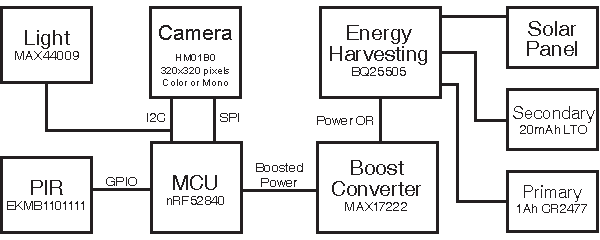
\includegraphics[width=\columnwidth]{figs/block_diagram.pdf}
\caption{\normalfont{\name system block diagram.
The system is based on the Himax HM01B0 camera and the Nordic NRF52840 MCU. We include a light and PIR sensor to provide a low power wake up mechanism to drive image capture. A hierarchical energy harvesting system with a rechargable and non-rechargable battery are utilized to provide a long, reliable lifetime to the system.
}}
\end{definefigure}

\begin{definefigure}{fig:arch}
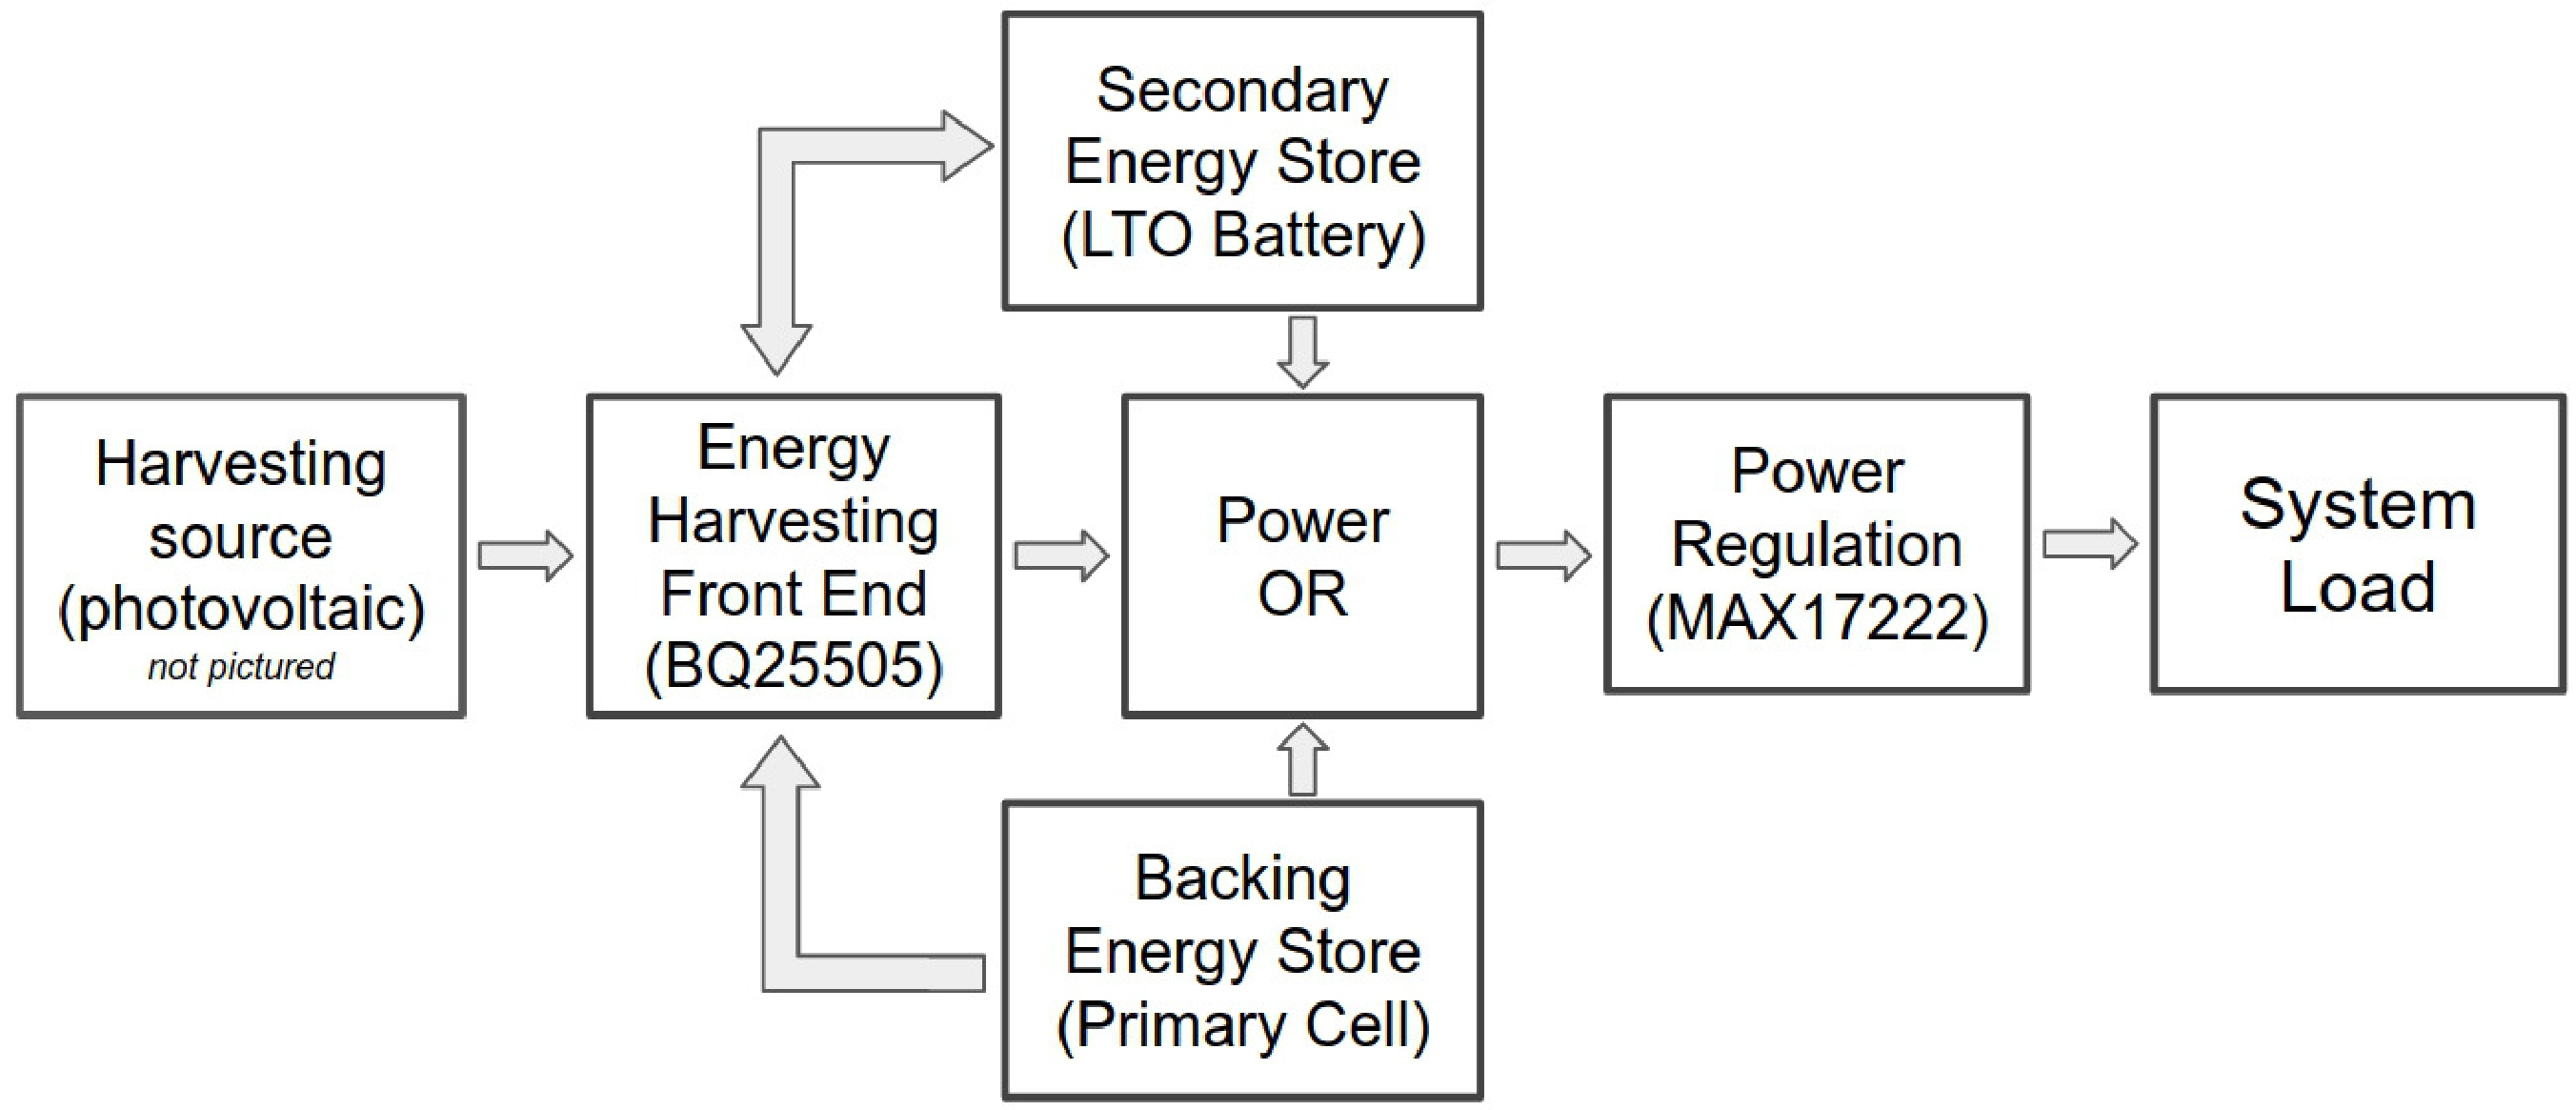
\includegraphics[width=0.85\columnwidth]{figs/arch.pdf}
\caption{\normalfont{The \name end-to-end image transfer architecture. \name uses Openthread, a 6LoWPAN network. This allows it to transmit images over the CoAP block protocol directly to any IP endpoint. We implement a CoAP server to recieve and reassemble image, demosaic them, and publish them over an MQTT stream. This CoAP server can be local to the sensors if privacy is desired. User applications running on PCs or on servers can easily subscribe to incoming images.}}
\end{definefigure}

\begin{definetable}{tab:components}
    \begin{threeparttable}
        \centering
        \footnotesize
        \begin{tabular}{l | l | c | c}
            Component                           & Function                     & Active Current          & Idle Current \\
            \hline
            Himax HM01B0                        & Image sensor                  & 2.0 mA                & 25.1\,\uA\,\tnote{a} \\
            \multirow{2}{*}{Nordic NRF52840}    & Processor                     & 52\,\uA/MHz           & 3.16\,\uA\,\tnote{b}  \\
                                                & Radio                         & 4.8\,mA @ 0\,dbm      & \textemdash\,\tnote{b}\\
            Ambiq AB1815-T3                     & Real time clock               & 55\,nA                & N/A\,\tnote{c}  \\
            Maxim MAX44009                      & Light sensor                  & 650\,nA               & N/A\,\tnote{c}  \\
            Panasonic EKMB11011                 & PIR Occupancy                 & 100\,\uA              & 1\,uA  \\
        \end{tabular}
    \end{threeparttable}
    \begin{tablenotes}[para]
    \scriptsize
    \item[a] Power gated when not in use.\\
    \item[b] Sleep current for both processor and radio, full RAM retention, wake on low freq. timer.\\
    \item[c] No shutdown or idle mode.
    \end{tablenotes}
    \vspace*{1mm}
    \caption{
    \normalfont
    The components used in \name. They represent some of the lowest power options currently available. Due to the extremely low idle power of all included components, \name is able to sleep at 4.4\uA.
    }
\end{definetable}

\begin{definefigure}{fig:demosaic}
\centering
\begin{subfigure}{0.49\columnwidth}
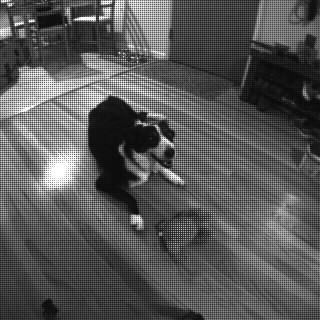
\includegraphics[width=\linewidth]{images/mosaic.jpeg}
\end{subfigure}
%
\begin{subfigure}{0.49\columnwidth}
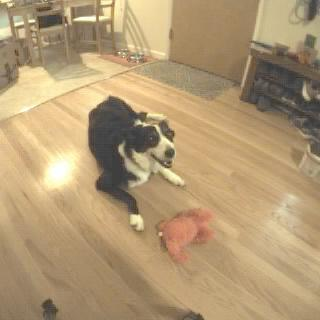
\includegraphics[width=\linewidth]{images/demosaic.jpeg}
\end{subfigure}
\caption{\normalfont{An image from \name, displayed as a mosaiced image (left) and demosaiced (right).}}
\end{definefigure}


\placefigure[t]{fig:block}

\section{Implementation}

In this section, we explore the implementation of \name{}, including component selection, techniques to enable a low power camera interface, and architectural details about the energy harvesting and storage architecture

We implement the design of \name{} in an \textbf{open source}\footnote{A link to project repository will be included on publication} hardware and software design. The platform is built around the Himax HM01B0 ultra low power camera \cite{hm01b0}. This camera has also enabled other platforms like BackCam \cite{josephson2019wireless} and Camaroptera \cite{nardello2019camaroptera}. The Himax camera is available in two different versions: monochrome and color. We use the color version of the sensor to ensure the ability to capture color information of images, but the two versions are pin compatible and can be interchanged. The other key component of the design is the SoC processor. We use the Nordic nRF52840 Cortex-M4F SoC as it is one of the most power efficient processors available, includes a Floating Point Unit (FPU), and is relatively fast compared to other low power microcontrollers at 64\,MHz. An FPU allows the platform to perform floating point dependent tasks like image compression. It has a multiprotocol BLE/802.15.4 radio that is well supported by OpenThread, an open source implementation of the Thread 6LoWPAN mesh network protocol. It features comparatively large amounts of flash (1\.MB) and SRAM (256\.kB), which is enough to capture images and perform some local processing. We include an ultra-low power real time clock (RTC) to provide accurate image timestamps. The platform also features an ultra low power PIR sensor and illuminance sensor to provide a low power wakeup mechanism and illuminance calibration for captured images. A block diagram of the major system components is displayed in \cref{fig:block}. Characteristics of the sensors and the MCU are summarized in \cref{tab:components}. In the next few sections we describe \name{}'s implementation, including the MCU to camera interface, energy harvesting architecture, image compression methods, the end-to-end image transmission architecture, and an implementation of onboard person classification.

\subsection{Camera Interface}
The majority of image sensors do not support normal sensor interfaces like I2C or SPI to transfer data. Instead they rely on high frequency ($\geq$8\,MHz) serial or parallel data busses. This is because images are many kilobytes or megabytes in size, and data transfer must be at a high frequency or parallel to transfer multiple frames per second. The majority of embedded processors, the nRF52840 included, are not designed to interface with parallel camera busses. Traditionally, platforms have used intermediate hardware like dedicated processors, CPLDs or FPGAs to interface with image sensors and buffer frames \cite{rowe2007firefly,rahimi2005cyclops}. The Himax HM01B0 has two interfaces, an I2C command interface and a serial, 4x, or 8x data interface.
The Himax HM01B0 requires an input master clock (MCLK) of 3-36\,MHz to drive internal sensor timings and outputs a pixel clock (PCLKO), and frame valid (FVLD) and line valid (LVLD) signals \cite{hm01b0}. It can be configured to capture full frame (320x320), QVGA (320x240), and if the mono version of the sensor, downscaled QQVGA (160x120) resolution images. In \name{} we capture full frame images and use the color version of the sensor. This version produces CFA images that must be demosaiced into a three channel RGB image. An example of a mosaiced image and its demosaiced counterpart is displayed in \cref{fig:demosaic}. \name{}'s processor does not possess enough memory to locally demosaic an image so any inference or transmission must be done with the mosaiced image. We power-gate the HM01B0 camera on \name, allowing the system to power the camera off and enter the lowest possible power state.

\placefigure[t]{tab:components}

Other systems that utilize the Himax HM01B0 camera including BackCam, Camaroptera, and the Sparkfun Edge have developed a bitbang protocol to emulate a parallel interface \cite{josephson2019wireless, nardello2019camaroptera, sparkfunedge}. This is possible because their processors support GPIO direct memory access (DMA). This allows the GPIO peripheral to directly write to memory, avoiding costly processor cycles to load GPIO state into registers and then write it to memory. This optimization allows a bitbang protocol on these platforms to operate faster than the HM01B0's minimum operating frequency. However, a bitbang protocol is undesirable because it requires the processor to be on during an image transfer, consuming additional energy. The nRF52840 does not support DMA GPIO. Because of this, developing a bitbang protocol that adheres to the required camera timing is infeasible. Instead, we note that the camera serial protocol closely resembles SPI, and the nRF52840 implements an 8\,MHz SPI peripheral with DMA support. The camera PCLKO signal is identical to SCLK, and can be gated by LVLD. The signal LVLD from the camera indicates when a line of the image is being transmitted, and is analogous to a SPI chip select line. However, this line is active high, and most SPI implementations, including the hardware on the nRF52840, expect active low. Inserting a low latency inverter in between the LVLD output of the camera and the MCU allows the nRF52840 SPI peripheral to interface with the camera. This has the added benefit of reducing power required to read in images as the processor can sleep while the SPI peripheral directly writes images to memory.

\subsection{Energy Harvesting and Storage}
The energy storage architecture for \name{} is built around the TI BQ25505, an ultra-low power energy harvesting front-end~\cite{bq25505}. It supports a backup cell, and seamlessly handles power transitions between it and the rechargeable storage. We use the BQ25505 with a 2.4\,V 10.9\,cm\textsuperscript{2} amorphous solar panel to charge a 2.4\,V 20\,mAh rechargeable Lithium Titanate Oxide (LTO) battery. The BQ25505 uses maximum power point tracking to optimize the amount of captured energy. We use a lithium 3\,V 1\,Ah CR2477 coin cell as a backup. The output of the BQ25505's power OR is boosted to the system voltage by a MAX17222 regulator to power all components under a single voltage domain.

\placefigure[t]{fig:demosaic}

\subsection{Image Compression}
To reduce energy and time required to transmit images, we employ JPEG compression on images prior to transmission. We use the Moodstocks JPEC encoder, a simple and portable monochrome JPEG encoder written in C \cite{moodstocks}. JPEG compression, like most DSP algorithms, relies heavily on floating point arithmetic. Due to its integrated FPU, \name{}'s processor is able to compress full resolution 320x320 images in 210\,ms.
This encoder is also used in Camaroptera \cite{nardello2019camaroptera}, although this platform is based on the MSP430, which lacks an FPU. It requires 25 s to compress an downsampled 160x120 image using floating point emulation, and 7s when JPEC is adapted to fixed point math. This fixed point adaptation also reduces image quality slightly. It is clear that a camera platform like \name{} benefits greatly from the inclusion of a faster, more capable processor.
The current configuration of \name captures color filter array (CFA) images. A CFA is an alternating "mosaic" of green-blue-green and red-green-red rows of pixels~\cite{bayer1976color}. Each pixel corresponds to a single color, and through post-processing known as "demosaicing", a three channel RGB image is generated from the single channel representation. An example of a mosaiced image and its demosaiced counterpart are displayed in \cref{fig:demosaic}.
JPEG is not designed to compress mosaic images. However, we find that monochrome compression with a high quality setting does not overly degrade image fidelity or color representation. We explore the effects of monochrome compression on \name's captured images further in \cref{eval:compression}.

\placefigure[t]{fig:arch}

\subsection{End-to-end Image Pipeline}
To support transmitting full images, we implement a full application stack based on standard IP-based protocols. This end-to-end image architecture is depicted in \cref{fig:arch}.
We choose to use OpenThread, an open source implementation of the Thread network protocol for \name devices. Thread is a 6LoWPAN mesh network, and allows packets to be sent end-to-end over a standard IP network. OpenThread also provides implementations of useful protocols like CoAP, SNTP, and DNS. 
CoAP is a lightweight restful protocol similar to HTTP, but over UDP \cite{shelby2014constrained}. 
On top of OpenThread's CoAP API, we implement the CoAP Block add-on feature. This allows us to fragment large data like an image across multiple CoAP payloads \cite{bormann2016block}. 
The choice to use CoAP block is a reluctant one however, and was based on the available implementations of reliable transfer protocols for low power networks.
\name image transmission is a perfect application for TCP, although TCP is rarely implemented for low power networks. TCP has been shown to be provide a 40\% higher throughput compared to CoAP block over an OpenThread network~\cite{kumar2020performant} over an OpenThread network. However, this implementation is not yet included in mainline OpenThread, limiting us to CoAP block.

\name captures an image, compresses it using JPEG, and transmits the image using a CoAP blockwise transfer. The CoAP block messages are sent to an endpoint that reassembles them, parses their contents, and publishes a JSON message over an MQTT broker. An application running on the endpoint listens for the transmitted mosaiced images, demosaics them, and republishes the color image for application use. High level applications wishing to interface with images captured by \name devices simply must subscribe to the relevant device topics to receive images. From there, the images can be processed in frameworks like OpenCV, Tensorflow, or Pytorch~\cite{tensorflow2015-whitepaper, pytorch,itseez2015opencv}.

In addition to our data backhaul pipeline, we implement an independent update server. \name devices arbitrarily poll the update server every 24 hours for a new application image. If a newer image exists, it downloads it over a CoAP blockwise transfer and applies it. This allows users to deploy new applications quickly across an entire deployment with minimal intervention.

\placefigure[t]{fig:size-time-energy}
\placefigure[t]{fig:compression}
\placefigure[t]{fig:ssim}
\placefigure[t]{fig:lifetime}

\subsection{Local Image Classification}
In addition to transmitting images, we also demonstrate the ability of the platform to perform local inference.
While performing local object detection appears out of reach of the capabilities of \name, image classification (with a limited number of classes) is not. 
To explore the capabilities of machine learning inference on \name,
we modify and train our own MobileNets v1 network to perform person classification. We then deploy it to \name's processor using TensorFlow Lite for Microcontrollers. 

The parameter flexibility of MobileNets v1 allows us to reduce the size of the model so it can fit on a microcontroller. We reduce the size of the network by reducing the depth of each convolutional layer by 75\% ($\alpha$ = .25).  
%\hl{cut some of model details if space needed: }
The model consists of a regular convolution with batch normalization followed by multiple depthwise separable convolutions~\cite{howard2017mobilenets}. 
%The result of the convolutions is passed through an average pooling layer and a dense layer of 2 units, resulting in a person and no person score. A kernel size of 3 is throughout all convolutions.
There is insufficient memory to perform the forward pass on full sized 320x320 images, so images need to be downscaled. We configure this network for different input image dimensions including 48, 72, 96, and 120.
We train this model for 80 epochs on the Visual Wake Word dataset~\cite{chowdhery2019visual} to achieve a validation accuracy of 78\%, compared to a 90\% accuracy with an unmodified MobileNet. The model weights require 230\.kB after post-training quantization and achieve an accuracy of 76\% for input images of size 120x120 when using TensorFlow in Python. We deploy this model on \name and evaluate its performance in \cref{eval:localinf}.
